% =====================================================================
% Energy spectrum across tasks and circuits.
%
% Argument: the Walsh energy spectrum varies systematically across
% tasks and circuit types. Real circuits carry 5-30% order-2 energy;
% random circuits carry near zero. Order-3+ energy rarely exceeds 5%,
% so interactions are predominantly pairwise.
%
% Status: v1 draft. Data from results/all_walsh_results.csv (60 sweeps).
% =====================================================================

\subsection{The interaction spectrum varies systematically across tasks}
\label{sec:energy-spectrum}

The Walsh--Hadamard decomposition partitions each circuit's total
variance into contributions from each interaction order: order-1
(individual head effects), order-2 (pairwise interactions), and
order-3+ (higher-order terms). We computed exhaustive $2^n$ coalition
sweeps for 60 circuit--task--ablation combinations across six tasks in
GPT-2 small: IOI, reverse token identification (RTI), greater-than,
induction, subject-verb agreement (SVA), and gendered pronoun
resolution. Circuits range from 5 to 15 heads and include those
discovered by activation patching, EAP, ACDC, Walsh-based selection,
and random head sets.

\medskip

{\small
\begin{tabular}{llcccc}
\toprule
Task & Circuits & Sweeps & Order-1 & Order-2 & Order-3+ \\
\midrule
IOI            & 7 (canonical, EAP, epistatic) & 14 & 0.82 & 0.15 & 0.03 \\
RTI            & 3 (incl.\ EAP)               &  6 & 0.81 & 0.13 & 0.06 \\
Greater-than   & 5 (known, ACDC)               & 10 & 0.92 & 0.07 & 0.01 \\
Induction      & 5 (known, ACDC)               & 10 & 0.90 & 0.08 & 0.02 \\
SVA            & 5 (known, ACDC)               & 10 & 0.95 & 0.05 & 0.00 \\
Gendered pronoun & 5 (known, ACDC)             & 10 & 0.99 & 0.01 & 0.00 \\
\midrule
Random (all tasks) & 6 random head sets        & 12 & 0.92 & 0.06 & 0.02 \\
\bottomrule
\end{tabular}
}

\medskip

\noindent Energy fractions are averages over real (non-random) circuits
within each task, rounded to two decimal places.

Three patterns emerge. First, the amount of pairwise interaction varies
by task: IOI and RTI circuits carry 13--15\% of their variance at
order~2, while gendered pronoun circuits carry approximately 1\%. The
variation reflects the structure of the task: IOI requires coordinated
attention routing across multiple head classes, whereas gendered pronoun
resolution can be solved by a small set of independently operating heads.

Second, order-3+ energy rarely exceeds 5\% for real circuits (5 of 48
non-random sweeps). The pairwise Walsh spectrum captures the dominant
interaction structure; higher-order terms contribute marginally. This
justifies focusing on order-2 coefficients: a sparse recovery of
$k = n + \binom{n}{2}$ coefficients captures the interaction structure
that matters.

Third, random head sets carry near-zero order-2 energy (average 6\%
across all tasks), confirming that the interaction structure of real
circuits reflects functional coupling rather than an artifact of the
measurement. The one exception is a random SVA circuit under zero
ablation (35\% order-2), where the ablation primitive creates spurious
interactions by zeroing heads that the remaining heads depend on for
LayerNorm scaling.

Figure~\ref{fig:energy-spectrum} visualizes these patterns.

\begin{figure}[t]
\centering
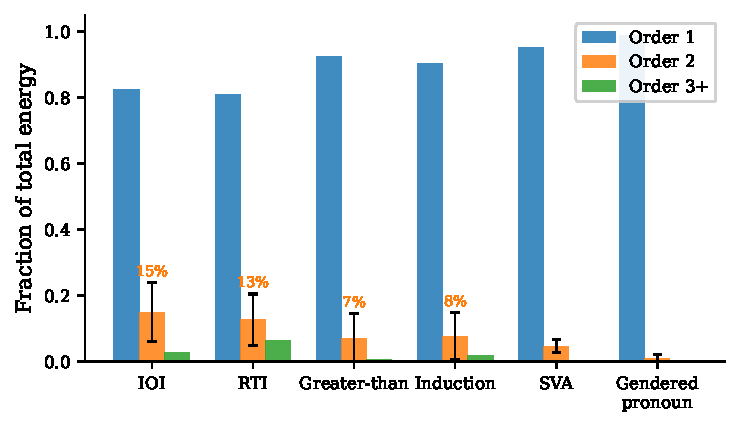
\includegraphics[width=0.75\textwidth]{figures/energy_spectrum.pdf}
\caption{Walsh energy spectrum across six tasks in GPT-2 small,
averaged over non-random circuits. IOI and RTI carry substantial
order-2 energy (13--15\%), indicating pairwise interactions that
additive circuit summaries discard. Gendered pronoun resolution is
nearly additive (${\sim}1\%$ order-2). Error bars show standard deviation
across circuits within each task.}
\label{fig:energy-spectrum}
\end{figure}
